\section{Design and Implementation}
\label{sec.design}

\subsection{Design of Our ``Secure Logging System''}
\label{sec.design.secure_logging_system}
Designing an implementation of the popular paths metric for use with containers required two separate tasks. 
First, we had to identify the popular paths for the underlying host operating system. 
And, second, once we knew where they were, second, we needed a way to log / block the non-popular paths to keep containers aways from these less-used 
and potentially buggy code paths. To address these issues, we came up with a dual module approach we call the Secure Logging System (Shown in Diagram \ref{fig:design}). 

\begin{figure*}
\centering
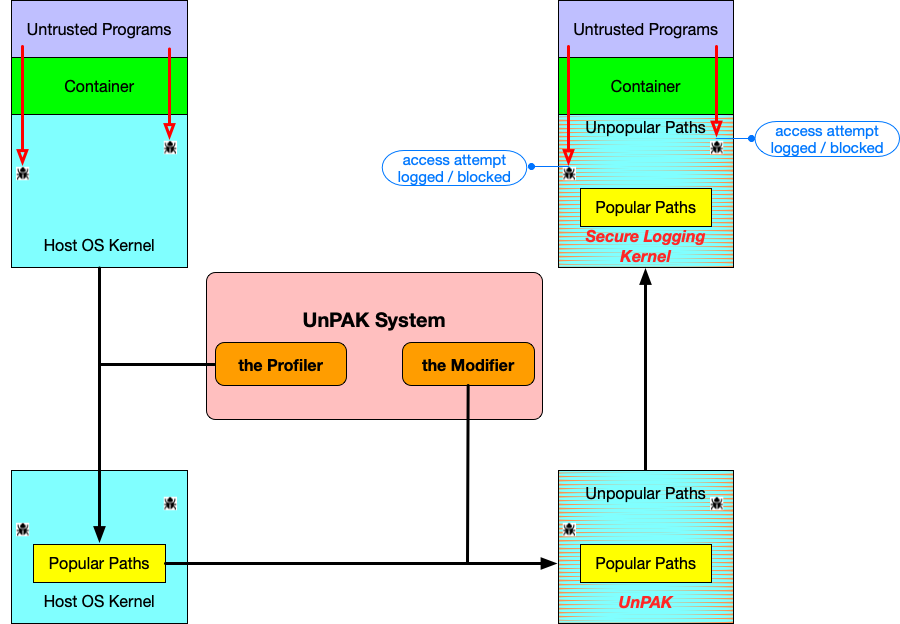
\includegraphics[width=1.5\columnwidth]{diagram/design.png}
\caption{\small Design Overview of Our Secure Logging System}
\label{fig:design}
\end{figure*}

Our system has two main modules, one is the ``Kernel Profiler'', the other one is the ``Kernel Modifier''. 
Our system operates in the following way: first, the Kernel Profiler will obtain the popular paths kernel trace for the given container system. 
Here, we define the ``popular paths kernel trace'' as the lines of code in the host kernel that are executed when running the default / regular workload 
(such workload is often defined in the configuration files that come with the container images) of a set of the most popular containers 
(ranked by the number of user downloads.) The key insight of our design is that this popular paths kernel trace we got should contain fewer kernel vulnerabilities, 
based on the findings in the Lock-in-Pop paper [3]. Second, our Kernel modifier leverages this popular paths data to enhance security of the kernel, 
by instrumenting the rarely used non-popular paths to either generate security warning messages, or block code execution on these potentially dangerous code paths. 
Finally, our Secure Logging System produces a Secure Logging Kernel, which is an instrumented Linux kernel with security checks inserted at the non-popular paths. 
This Secure Logging Kernel can then be used to run containers without any changes to the containers themselves, and help prevent kernel vulnerabilities from being triggered. 

\subsection{Implementation}
\label{sec.design.implementation}
Our Secure Logging System has two main modules, the Kernel Profiler and the Kernel modifier. We now describe how each of them was implemented. 

\subsubsection{Implementation of the Kernel Profiler}
\label{sec.design.implementation.kernel_profiler}
The Kernel Profiler is designed to collect the kernel trace of running user containers. 
Especially, we are interested in obtaining the popular paths kernel trace. 
In this work, the popular paths kernel trace refers to the lines of code in the underlying host operating system kernel that were executed when running the regular workload 
(defined in the configuration files of the corresponding container images) of popular (determined by the number of user downloads) containers. 
In our implementation, we chose to run our Kernel Profiler on popular Docker containers from Docker Hub [4]. 
Docker Hub provides millions of Docker container images, and the popular ones are downloaded more than ten millions times. 
Our Kernel Profiler works in the following way: 
\begin{enumerate}
	\item The Linux kernel used to run the Docker containers will first be recompiled with the Gcov [17] kernel profiling feature enabled. 
	\item Our Kernel Profiler used the LinuxKit toolkit to run the Docker containers on the Gcov-enabled Linux kernel. 
	To run the Docker containers, the Kernel Profiler first generate the configuration file for LinuxKit, in which the task container will be defined, 
	along with a data container responsible for collecting, storing, and transferring the kernel trace data. 
	\item When booting the LinuxKit virtual machine, the Kernel Profiler has a script to start running the workload of the task container. 
	And then, the Kernel Profiler will collect the kernel trace data (gcda files generated by Gcov), stored at ``/sys/kernel/debug/gcov'', 
	and transfer the data to the host system for further use. 
	\item From the host system, our Kernel Profiler used the lcov [18] tool to process the kernel trace data we collected, 
	and will generate the formatted data about which lines of code were executed in the kernel source files, to be used by our Kernel Modifier. 
\end{enumerate}

\begin{figure*}
\centering
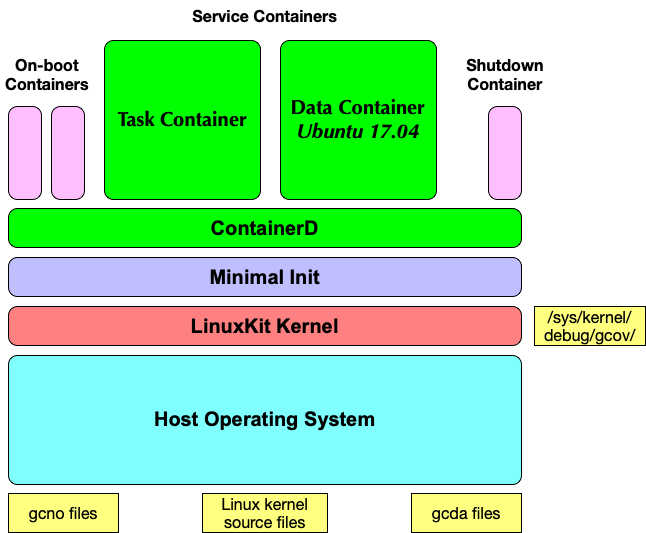
\includegraphics[width=1.5\columnwidth]{diagram/linuxkit-kernel-profiler.png}
\caption{\small Implementation of the Kernel Profiler}
\label{fig:linuxkit-kernel-profiler}
\end{figure*}

\subsubsection{Implementation of the Kernel Modifier}
\label{sec.design.implementation.kernel_modifier}
The Kernel Modifier is responsible for modifying the Linux kernel to insert security logging code at the non-popular paths. 
It needs to first identify the correct places in the Linux kernel source tree to be instrumented, and then perform the code modification. 
The Kernel Modifier has three main parts, the Clang compiler, the Clang analyzer, and the kernel instrumenting tool (shown in Diagram 3). 
It operates in the following way: 
\begin{enumerate}
	\item First, we used the Clang C compiler from the Clang / LLVM project [19] along with BEAR [20] tool to compile the Linux kernel source. 
	BEAR can help us generate a compilation database, which contains all the compile flags and options used during the kernel compilation process. 
	And this compilation database will be used by our Clang analyzer to perform source code parsing in our next step. 
	\item Once we got the compilation database for the Linux kernel, next, we used our Clang analyzer to perform static analysis on the kernel source code to obtain 
	the control flow graph for each function in the source code files. Our Clang analyzer leveraged Clang’s LibTooling [21] to construct the AST tree from the kernel source code, 
	and then obtain the control flow graph. From the control flow graph, we can identify the corresponding source line number for each basic block. 
	And the beginning lines of all the basic blocks in the source files are our candidates for adding security logging code at this point. 
	\item Next, our kernel instrumenting tool will perform the actual kernel modification based on the basic blocks we obtained, and the popular paths data we collected. 
	The algorithm for our kernel modification is that we go through the basic blocks in the kernel source files. If none of the lines in a basic block was in the popular paths data, 
	we consider this basic block as a non-popular basic block, and our kernel instrumenting tool will add the security logging code at the beginning of this non-popular basic block. 
	One optimization strategy we conducted here is that if we discover that an entire function has none of its lines in the popular paths data, 
	we consider this function as a non-popular function, and then we just add our security logging code once at the beginning of this function, 
	avoiding adding redundant and unnecessary code inside this function. 
	\item Finally, our Kernel Modifier will produce the Secure Logging Kernel. And It can be directly used to run Docker containers in the LinuxKit VM. 
\end{enumerate}

\begin{figure*}
\centering
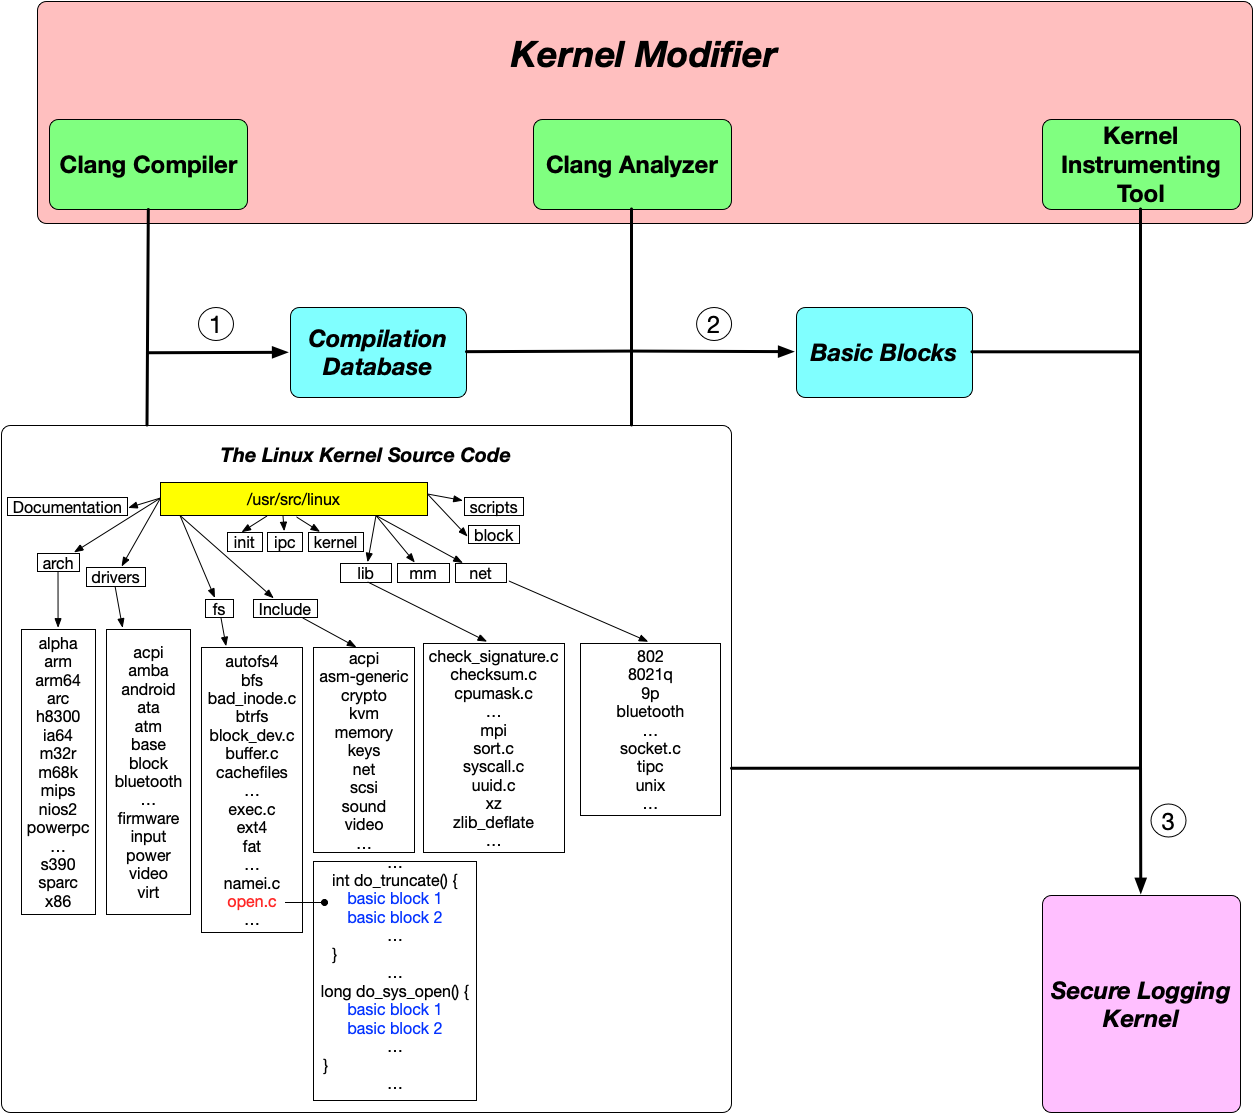
\includegraphics[width=1.5\columnwidth]{diagram/linuxkit-kernel-modifier.png}
\caption{\small Implementation of the Kernel Modifier}
\label{fig:linuxkit-kernel-modifier}
\end{figure*}
